\documentclass[border=1pt]{standalone}
\usepackage{tikz}
\usetikzlibrary{calc}
\usepackage{gensymb}
\usepackage{palatino}
\usetikzlibrary{intersections}

\begin{document}
\footnotesize
\noindent
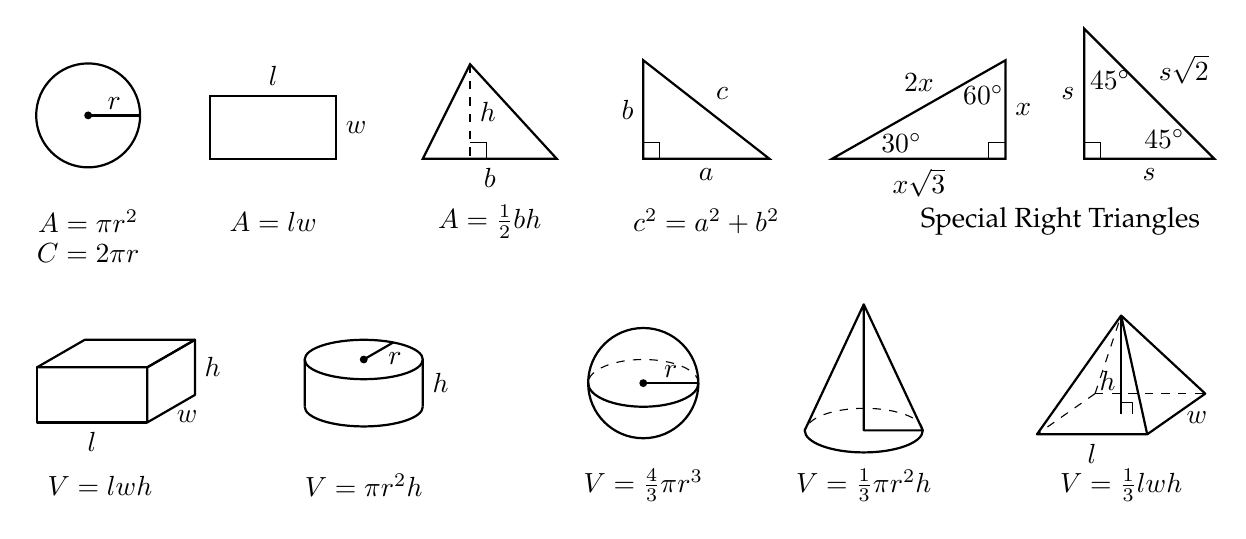
\begin{tikzpicture}[scale=1.0]

%%%%%%%%%%%%%%%%%%%%%%%%%%%%%%%%%%%%%%%%%%%%%%
% Circle
%%%%%%%%%%%%%%%%%%%%%%%%%%%%%%%%%%%%%%%%%%%%%%
\begin{scope}[xshift=0cm]
\def\xcen{0.65}
\def\ycen{0.55}
\def\rad{0.66}
\draw[thick] (\xcen,\ycen) circle (\rad) coordinate (center);
\draw[thick] (center) --++(0:\rad) node[midway,above,yshift=-0.5mm] {$r$};
\fill (center) circle [radius=0.05cm];
\end{scope}

%%%%%%%%%%%%%%%%%%%%%%%%%%%%%%%%%%%%%%%%%%%%%%
% Rectangle
%%%%%%%%%%%%%%%%%%%%%%%%%%%%%%%%%%%%%%%%%%%%%%
\begin{scope}[xshift=0cm]
\def\xstart{2.2}
\def\ystart{0.0}
\def\xlen{1.6}
\def\ylen{0.8}
\pgfmathsetmacro{\xend}{\xstart+\xlen}
\pgfmathsetmacro{\yend}{\ystart+\ylen}
\draw[thick] (\xstart,\ystart) -- (\xstart,\yend) -- (\xend,\yend) coordinate[midway] (xmid) -- (\xend,\ystart) coordinate[midway] (ymid) -- cycle;
\node[above] at (xmid) {$l$};
\node[right] at (ymid) {$w$};
\coordinate (nodetext) at ([yshift=-16mm]xmid) ;
% add formula 
\node at (nodetext) {$A=lw$};
\end{scope}

%%%%%%%%%%%%%%%%%%%%%%%%%%%%%%%%%%%%%%%%%%%%%%
% Triangle
%%%%%%%%%%%%%%%%%%%%%%%%%%%%%%%%%%%%%%%%%%%%%%
\begin{scope}[xshift=0cm]
\def\xa{4.9}
\def\ya{0.0}
\def\xlen{1.7}
\def\xfirst{0.6}
\def\height{1.2}
\def\yc{2.4}
\def\rasize{6pt}
\draw[thick] (\xa,\ya) coordinate (start) -- ++(\xlen,0) coordinate[midway] (xmid) -- ($(\xa,\ya)+(\xfirst,\height)$) coordinate (top) -- cycle;
\node[below] at (xmid) {$b$};
\coordinate (base) at (top |- start);
\draw[dashed] (top) -- (base) coordinate[midway] (ymid);
\node[right] at (ymid) {$h$};
% right angle symbol
\draw ([xshift=\rasize]base) -- ++(0,\rasize) -- ++(-\rasize,0);
% add formula 
\path let \p1=(nodetext), \p2=(xmid) in (\x2,\y1) node {$A=\frac{1}{2}bh$};
% add formulae for circle
\path let \p1=(nodetext), \p2=(center) in (\x2,\y1) node {$A=\pi r^2$};
\path let \p1=(nodetext), \p2=(center) in (\x2,\y1) node[yshift=-4mm] {$C=2 \pi r$};
\end{scope}

%%%%%%%%%%%%%%%%%%%%%%%%%%%%%%%%%%%%%%%%%%%%%%
% 3-4-5 Triangle
%%%%%%%%%%%%%%%%%%%%%%%%%%%%%%%%%%%%%%%%%%%%%%
\begin{scope}[xshift=0cm]
\def\xa{7.7}
\def\ya{0.0}
\def\xlen{1.6}
\def\height{1.25}
\def\rasize{6pt}
% set up coordinates
\coordinate (A) at (\xa,\ya);
\coordinate (B) at ($(A)+(0,\height)$);
\coordinate (C) at ($(A)+(\xlen,0)$);
% draw triangle
\draw[thick] (A) -- (B) -- (C) -- cycle;
% labels
\path (A) -- (B) node[midway,left] {$b$};
\path (B) -- (C) node[midway,above right] {$c$};
\path (C) -- (A) node[midway,below] (mid) {$a$};
% right angle symbol
\draw ([xshift=\rasize]A) -- ++(0,\rasize) -- ++(-\rasize,0) -- ++(0,-\rasize);
% add formula 
\path let \p1=(nodetext), \p2=(mid) in (\x2,\y1) node {$c^2 = a^2 + b^2$};
\end{scope}

%%%%%%%%%%%%%%%%%%%%%%%%%%%%%%%%%%%%%%%%%%%%%%
% 30-60-90 Triangle
%%%%%%%%%%%%%%%%%%%%%%%%%%%%%%%%%%%%%%%%%%%%%%
\begin{scope}[xshift=0cm]
\def\xa{10.1}
\def\ya{0.0}
\def\xlen{2.2}
\def\height{1.25}



%\def\xb{14.9}
%\def\ya{2.2}
%\def\yb{3.35}
\def\rasize{6pt}
% set up coordinates
\coordinate (A) at (\xa,\ya);
\coordinate (B) at ($(A)+(\xlen,0)$);
\coordinate (C) at ($(B)+(0,\height)$);
% draw triangle
\draw[thick] (A) -- (B) -- (C) -- cycle;
% labels
\path (C) -- (A) node[midway,above,yshift=1mm] {$2x$};
\path (B) -- (C) node[midway,right] {$x$};
\path (A) -- (B) node[midway,below] (mid) {$x\sqrt{3}$};
\node[right] (tmp) at ([xshift=5mm,yshift=2mm]A) {$30\degree$};
\node[below left] (tmp) at ([xshift=1mm,yshift=-2mm]C) {$60\degree$};
%\draw (B) -- (A) -- (C)	pic[""] (alpha) {angle=B--A--C} ;
%\draw ([xshift=0cm,yshift=0cm]alpha) node  {$x\degree$};
% right angle symbol
\draw ([xshift=-\rasize]B) -- ++(0,\rasize) -- ++(\rasize,0);
% add formula 
\path let \p1=(nodetext), \p2=(mid) in (\x2,\y1) node[anchor=west,xshift=-1mm] {Special Right Triangles};
\end{scope}


%%%%%%%%%%%%%%%%%%%%%%%%%%%%%%%%%%%%%%%%%%%%%%
% Isosceles Triangle
%%%%%%%%%%%%%%%%%%%%%%%%%%%%%%%%%%%%%%%%%%%%%%
\begin{scope}[xshift=0cm]
\def\xa{13.3}
\def\ya{0.0}
\def\xlen{1.65}
\def\height{1.65}

%\def\xb{17.0}
%\def\ya{2.2}
%\def\yb{3.65}
\def\rasize{6pt}
% set up coordinates
\coordinate (A) at (\xa,\ya);
\coordinate (B) at ($(A)+(\xlen,0)$);
\coordinate (C) at ($(A)+(0,\height)$);
% draw triangle
\draw[thick] (A) -- (B) -- (C) -- cycle;
% labels
\path (A) -- (B) node[midway,below] {$s$};
\path (B) -- (C) node[midway,above right] {$s\sqrt{2}$};
\path (C) -- (A) node[midway,left] (mid) {$s$};
\node[below right] (tmp) at ([xshift=-0.5mm,yshift=-4mm]C) {$45\degree$};
\node[above left] (tmp) at ([xshift=-2.5mm,yshift=0mm]B) {$45\degree$};
% right angle symbol
\draw ([xshift=\rasize]A) -- ++(0,\rasize) -- ++(-\rasize,0);
\end{scope}



%%%%%%%%%%%%%%%%%%%%%%%%%%%%%%%%%%%%%%%%%%%%%%
% Rectangle Volume
%%%%%%%%%%%%%%%%%%%%%%%%%%%%%%%%%%%%%%%%%%%%%%
\begin{scope}[xshift=0cm,line join=round]
\def\xa{0.0}
\def\ya{-3.35}

\def\xlen{1.4}
\def\height{0.7}
\def\depth{0.7}

\def\angle{30}

%\def\xb{6.8}
%\def\xc{7.6}
%\def\xd{8.1}
%\def\ya{2.45}
%\def\yb{2.75}
%\def\yc{3.1}
%\def\yd{3.4}
% front corners
\coordinate (A1) at (\xa,\ya);
\coordinate (B1) at ($(A1)+(\xlen,0)$);
\coordinate (C1) at ($(B1)+(0,\height)$);
\coordinate (D1) at ($(A1)+(0,\height)$);
%back corners
\coordinate (B2) at ($(B1)+(\angle:\depth)$);
\coordinate (C2) at ($(C1)+(\angle:\depth)$);
\coordinate (D2) at ($(D1)+(\angle:\depth)$);
% draw three rectangles
\draw[thick] (A1) -- (B1) coordinate[midway] (xmid) -- (C1) -- (D1) -- cycle;
\draw[thick] (B1) -- (B2) -- (C2) -- (C1) -- cycle;
\draw[thick] (C1) -- (C2) -- (D2) -- (D1) -- cycle;
% label the sides
\path (A1) -- (B1) node[midway,below] {$l$};
\path (B1) -- (B2) node[midway,below right,xshift=-0.5mm,yshift=1mm] {$w$};
\path (B2) -- (C2) node[midway,right] {$h$};
% add formula for volume
\coordinate (nodetext) at ([yshift=-8mm]xmid) ;
\path let \p1=(nodetext), \p2=(nodetext) in (\x2,\y1) node[xshift=1mm] {$V=lwh$};
\end{scope}


%%%%%%%%%%%%%%%%%%%%%%%%%%%%%%%%%%%%%%%%%%%%%%
% Cylinder Volume
%%%%%%%%%%%%%%%%%%%%%%%%%%%%%%%%%%%%%%%%%%%%%%
\begin{scope}[xshift=0cm,line join=round]
\def\xcen{4.15}
\def\ycen{-2.55}
\def\xmajor{0.75}
\def\xminor{0.25}
\def\len{0.8}
\def\ycennew{\ycen-\len}
% define coordinates
\coordinate (cen) at (\xcen,\ycen);
\coordinate (A) at ($(cen)+(180:{\xmajor} and {\xminor})$);
\coordinate (B) at ($(cen)+(0:{\xmajor} and {\xminor})$);
% add top ellipse
\draw[thick] (cen) ellipse ({\xmajor} and {\xminor}) ;
% add lines at the side
\draw[thick] (A) -- ($(A)!\len!-90:(cen)$) coordinate (A1);
\draw[thick] (B) -- ($(B)!\len!90:(cen)$) coordinate (B1);
\path (B) -- ($(B)!\len!90:(cen)$) coordinate[midway] (mid);
\node[right] at (mid) {$h$}; 
% add lower arc
%\draw[thick] (B1) arc (0:-180:{\xmajor} and {\xminor}) ;
\draw[thick] (B1) arc (0:-180:{\xmajor} and {\xminor}) ;
% add dot in the middle
\fill (cen) circle [radius=0.05cm];
% add radius
\draw[thick] (\xcen,\ycen) -- ++(60:{\xmajor} and {\xminor}) coordinate[midway] (mid);
\node [yshift=1mm,below right] at (mid) {$r$};
% add formula 
\path let \p1=(nodetext), \p2=(cen) in (\x2,\y1) node {$V=\pi r^2 h$};
\end{scope}


%%%%%%%%%%%%%%%%%%%%%%%%%%%%%%%%%%%%%%%%%%%%%%
% Sphere Volume
%%%%%%%%%%%%%%%%%%%%%%%%%%%%%%%%%%%%%%%%%%%%%%
\begin{scope}[xshift=0cm,line join=round]
\def\xcen{7.7}
\def\ycen{-2.85}
\def\radius{0.7}
\def\xminor{0.3}
% define coordinates
\coordinate (cen) at (\xcen,\ycen);
\coordinate (left) at ($(cen)-(\radius,0)$);
\coordinate (right) at ($(cen)+(\radius,0)$);
% add arcs
\draw[thick] (right) arc (0:-180:{\radius} and {\xminor}) ;
\draw[dashed] (right) arc (0:180:{\radius} and {\xminor}) ;
% add circle
\draw[thick] (cen) circle [radius = \radius];
% add dot in the middle
\fill (cen) circle [radius=0.05cm];
% add radius
\draw[thick] (\xcen,\ycen) -- ++(0:\radius) coordinate[midway] (mid);
\node [yshift=-0.5mm,above] at (mid) {$r$};
% add formula 
\path let \p1=(nodetext), \p2=(cen) in (\x2,\y1) node {$V=\frac{4}{3} \pi r^3$};
\end{scope}

%%%%%%%%%%%%%%%%%%%%%%%%%%%%%%%%%%%%%%%%%%%%%%
% Cone Volume
%%%%%%%%%%%%%%%%%%%%%%%%%%%%%%%%%%%%%%%%%%%%%%
\begin{scope}[xshift=0cm,line join=round]
\def\xcen{10.5}
\def\ycen{-3.45}
\def\radius{0.75}
\def\xminor{0.28}
\def\height{1.6}
% define coordinates
\coordinate (cen) at (\xcen,\ycen);
\coordinate (left) at ($(cen)-(\radius,0)$);
\coordinate (right) at ($(cen)+(\radius,0)$);
\coordinate (top) at ($(cen)+(0,\height)$);
% draw solid line
%\draw (left) -- (top) -- (right) -- (cen) -- (top);

\draw[thick] (right) -- (cen) -- (top) -- 
	(right)  arc (0:-180:{\radius} and {\xminor}) 
	-- (top) -- cycle;
% draw dashed arc
%\draw (right) arc (0:-180:{\radius-0.01} and {\xminor}) ;
\draw[dashed] (right) arc (0:180:{\radius-0.01} and {\xminor}) ;
%\draw[dashed] (right) arc (0:180:{\radius} and {\xminor}) ;
%% add cone
%\draw (left) -- (top) -- right;
%% add height
%\draw (cen) -- (top);
%% add dot in the middle
%\fill (cen) circle [radius=0.05cm];
%% add radius
%\draw (\xcen,\ycen) -- ++(0:\radius) coordinate[midway] (mid);
%\node [yshift=-0.5mm,above] at (mid) {$r$};
% add formula 
\path let \p1=(nodetext), \p2=(cen) in (\x2,\y1) node {$V=\frac{1}{3} \pi r^2 h$};
\end{scope}

%%%%%%%%%%%%%%%%%%%%%%%%%%%%%%%%%%%%%%%%%%%%%%
% Pyramid Volume
%%%%%%%%%%%%%%%%%%%%%%%%%%%%%%%%%%%%%%%%%%%%%%
\begin{scope}[xshift=0cm,line join=round]
\def\xa{12.7}
\def\ya{-3.5}
\def\xlen{1.4}
\def\depth{0.9}
\def\angle{35}
\def\height{1.25}
\def\rasize{4pt}

% define coordinates
\coordinate (A) at (\xa,\ya);
\coordinate (B) at ($(A)+(\xlen,0)$);
\coordinate (C) at ($(B)+(\angle:\depth)$);
\coordinate (D) at ($(C)+(-\xlen,0)$);
\path[name path=A--C] (A) -- (C);
\path[name path=B--D] (B) -- (D);
\path [name intersections={of=A--C and B--D,by=cen}];
\coordinate (top) at ($(cen)+(0,\height)$);
% draw solid lines
\draw[thick] (top) -- (A) -- (B) node[midway,below] {$l$} -- (C) node[midway,right,yshift=-0.5mm] {$w$} -- (top) -- (B);
% draw height
\draw[thick] (cen) -- (top) node[midway,left,xshift=0.6mm,yshift=-2mm] {$h$};
% draw dashed lines
\draw[dashed] (D) -- (C);
\draw[dashed] (D) -- (top);
\draw[dashed] (D) -- (A);
% right angle symbol
\draw ([xshift=\rasize]cen) -- ++(0,\rasize) -- ++(-\rasize,0);
% add formula 
\path let \p1=(nodetext), \p2=(cen) in (\x2,\y1) node {$V=\frac{1}{3} l w h$};
\end{scope}





\end{tikzpicture}

\end{document}
